\chapter{Introducción}
\label{cap:introduccion}

\section{De los primeros pasos a la revolución del transformador}

En 1950, Alan Turing publicó un trabajo fundacional que cambió para siempre cómo pensamos 
sobre máquinas inteligentes. Propuso el Test de Turing: una prueba donde un interrogador humano conversa por 
escrito con dos entidades sin saber cuál es persona y cuál máquina. Si la máquina logra ser indistinguible de un 
humano, ha demostrado verdadera inteligencia. La genialidad de esta idea no estaba en medir cuánto sabía la máquina,
sino en evaluar si podía pensar y comunicarse de forma similar a nosotros. Pero Turing fue mucho más allá: en ese 
mismo trabajo introdujo conceptos que parecían ciencia ficción en su época: aprendizaje automático, donde máquinas 
mejoran con la experiencia; algoritmos genéticos, inspirados en evolución natural; y 
aprendizaje por refuerzo, donde máquinas aprenden por ensayo y error. Estas ideas sembraron una revolución que 
aún hoy continúa.

Mientras Turing escribía estas visiones futuristas, otros investigadores ya exploraban 
caminos paralelos. En 1943, Warren McCulloch y Walter Pitts publicaron un trabajo pionero que formalizó 
matemáticamente cómo funcionaba una neurona artificial. Inspirándose en la biología del cerebro pero usando 
lógica rigurosa, propusieron el primer modelo formal qué permitía a máquinas procesar información y 
aprender, no mediante reglas explícitas sino a través de patrones en los datos. Esta fue la chispa que encendería 
el fuego de las redes neuronales.


Seis años después de Turing, en 1956, sucedió algo crucial: investigadores como John McCarthy, Marvin Minsky, 
Allen Newell y Herbert Simon se reunieron en una conferencia en Dartmouth College que marcaría el nacimiento 
oficial de la Inteligencia Artificial como disciplina formal. El optimismo era contagioso. Estos investigadores
creían que cualquier aspecto de la inteligencia humana podía ser descrito con precisión matemática y, por tanto, 
simulado en una máquina. Algunos predijeron audazmente que en apenas diez años tendríamos máquinas tan inteligentes
como los humanos. 

Mientras unos perseguían razonamiento lógico puro, otros exploraban un enfoque radicalmente diferente: redes 
neuronales que pudieran aprender del mundo. Frank Rosenblatt presentó el perceptrón en 1958, una máquina que 
demostraban que era posible construir algoritmos que mejoraban con la práctica, tal como lo hacemos los humanos. 
Los periódicos hablaban del futuro prometedor de estas máquinas pensantes; la publicidad hablaba de máquinas que caminarían, hablarían y serían conscientes de su existencia. El 
entusiasmo era casi ilimitado.

\begin{figure}[t!] 
    \centering      
    \subfloat[Mark I Perceptron en el Laboratorio Aeronáutico de Cornell]{
        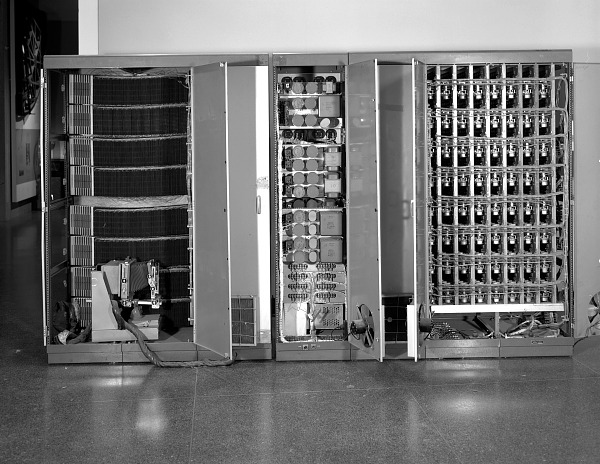
\includegraphics[height=6cm]{Imagenes/mark_perceptron_full2.jpg}
    } 
    \hfill
    % --- FRANK ROSENBLATT (Ya no es un histograma) ---
    \subfloat[Frank Rosenblatt ajustando el cableado del Perceptron.\label{subfig:frank}]{
        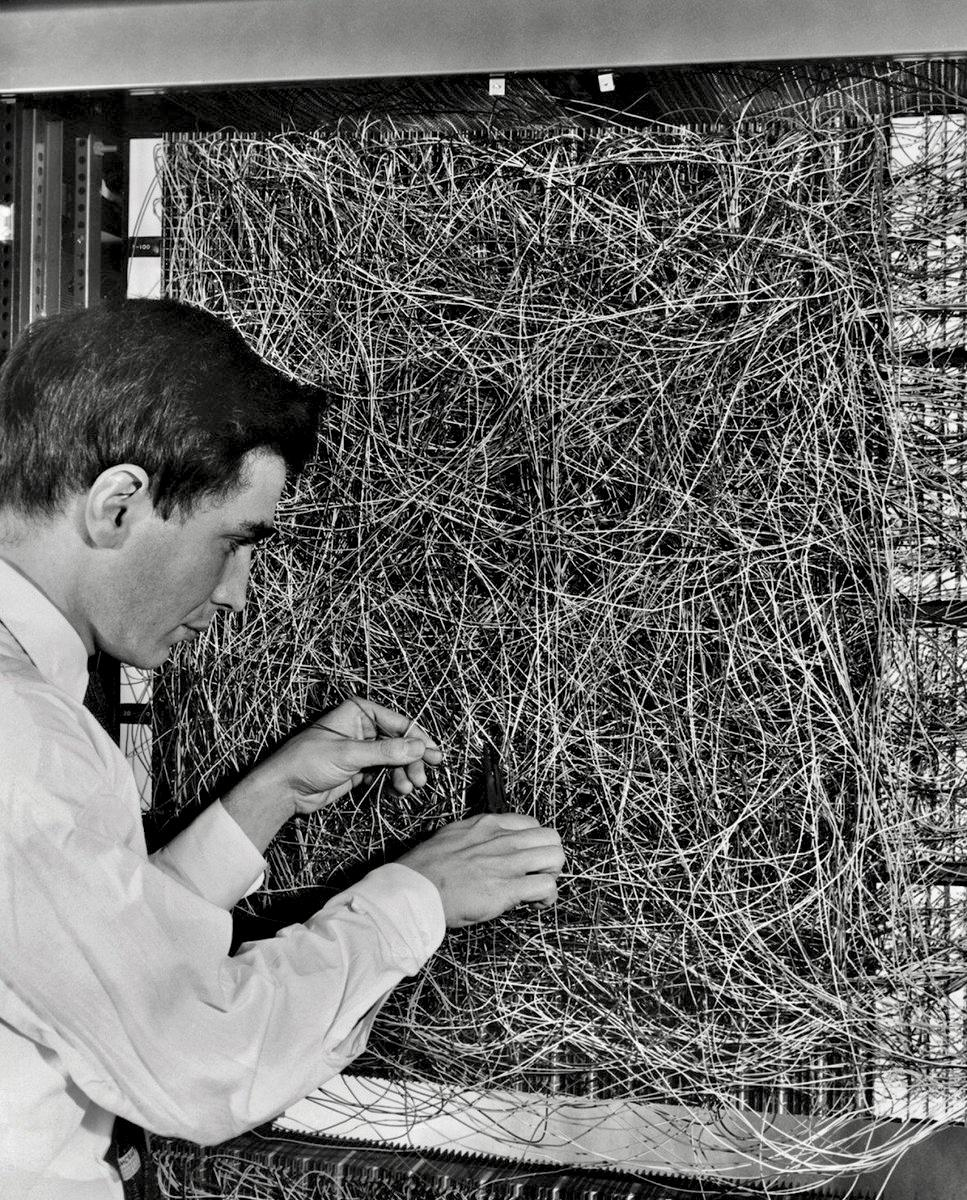
\includegraphics[height=6cm]{Imagenes/frank.jpg}
    }

    \caption{A la izquierda, el perceptron creado por Frank Rosenblatt llamado \textit{Mark I Perceptron}. 
    A la derecha, Frank Rosenblatt trabajando en las conexiones del perceptrón.}
    \label{fig:perceptron} 
\end{figure}

Pero la realidad es más compleja que las predicciones. En 1969, Marvin Minsky y Seymour Papert publicaron un 
análisis matemático devastador demostrando que los perceptrones simples tenían limitaciones fundamentales 
insuperables: había problemas que simplemente no podían resolver. Este descubrimiento fue como una ducha de agua 
fría. La financiación se redujo drásticamente, los periódicos perdieron interés y muchos investigadores abandonaron el 
campo.

Afortunadamente, el resurgimiento llegó en los años 1980s. Investigadores de múltiples grupos, trabajando de
forma independiente, redescubrieron el algoritmo de retropropagación, una técnica
elegante para entrenar redes neuronales profundas con múltiples capas. De repente, era posible entrenar redes
mucho más complejas.

Durante los años siguientes, especialmente en los 2000s y 2010s, el campo experimentó una evolución 
espectacular impulsado por tres factores: la disponibilidad de enormes volúmenes de datos en internet, el aumento de 
la capacidad computacional (especialmente el uso de unidades gráficas o \textit{GPUs}), y algoritmos más sofisticados. 
Esto dio lugar a la era del aprendizaje profundo (\textit{deep learning}), donde redes neuronales con muchas capas 
lograron hazañas extraordinarias en reconocimiento de imágenes y juegos complejos. Sin embargo, cuando se trataba de 
procesar lenguaje y secuencias de texto, la mejor solución seguía siendo las redes neuronales 
recurrentes (\textit{RNNs}), que procesaban información palabra por palabra. Pero estas redes tenían un talón de Aquiles:
la información crucial se perdía conforme procesaban secuencias más largas y sin capacidad de paralelismo, lo que 
resultaba en sistemas lentos e ineficientes.

En 2017, un equipo de investigadores de Google publicó un trabajo titulado ``\textit{Attention Is All You Need}''
que introdujo el transformador: una arquitectura basada en un mecanismo de autoatención (\textit{self-attention}) 
que permitía procesar todas las palabras de una secuencia simultáneamente en lugar de una a una. 
Aunque parecía un cambio técnico menor, sus consecuencias fueron revolucionarias.

De esta arquitectura brotaron los modelos extensos de lenguaje (\textit{Large Language Models}, LLMs): GPT, BERT,
Gemini y otros. Estos sistemas, entrenados con cantidades masivas de texto de internet, desarrollaron capacidades
que parecían imposibles años atrás. Pueden escribir ensayos convincentes, traducir entre idiomas preservando
significado, generar código de programación, y explicar conceptos complejos de formas que un estudiante puede 
entender. El salto cualitativo en estas capacidades ha sido tan alto que ha reconfigurado completamente campos 
como la traducción automática, el reconocimiento de voz, el análisis médico y la investigación científica. 
Pero la revolución va mucho más allá de lo técnico, pues estos modelos están presentes en nuestra vida cotidiana y 
su mayor logro es su asombrosa facilidad de uso, ya que al interactuar directamente mediante un lenguaje natural 
han derribado las barreras digitales tradicionales, permitiendo así que cualquier persona, incluso personas 
mayores o personas completamente ajenas a la tecnología, los utilicen a diario de forma intuitiva. 
Al facilitar el acceso a estas herramientas, no solo han transformado cómo escribimos o cómo trabajamos sino también
cómo interactuamos con el conocimiento.

Sin embargo, a pesar de que miles de millones de personas usan estas tecnologías diariamente, relativamente pocos 
entienden realmente cómo funcionan. La mayoría interactúa con estos sistemas como
si fueran cajas mágicas, sin comprender los principios matemáticos que subyacen a su funcionamiento y, lo peor de todo, que toman
estos modelos como fuentes fiables de información.

\section{Objetivos de este trabajo}

El objetivo central de este trabajo es construir paso a paso una comprensión integral de cómo funcionan los 
transformadores, de tal forma que quien lo lea pueda apreciar los principios matemáticos y conceptuales que subyacen 
a estas tecnologías.

Para lograrlo, en primer lugar se estudiará la fundamentación teórica de las redes neuronales, estableciendo 
los cimientos conceptuales necesarios para comprender arquitecturas más sofisticadas. Posteriormente, se analizará en 
profundidad la arquitectura del transformador y su mecanismo central de autoatención, explicando de qué forma esta 
innovación supera las limitaciones críticas de los modelos recurrentes clásicos y revoluciona el procesamiento de 
secuencias al permitir el paralelismo computacional.

A continuación, se explorará cómo los transformadores transformaron el procesamiento del lenguaje natural que 
originaron los modelos extensos de lenguaje (LLMs), estudiando los procesos clave que hacen posible que estos sistemas generen 
lenguaje coherente y contextualmente apropiado. Finalmente, se implementará un transformador tipo 
codificador-decodificador para traducción automática, demostrando que los principios teóricos explicados poseen 
validez práctica cuando se aplican a problemas tangibles del mundo real.
